\subsection{Ground Sample Distance - GSD}
%se litt på
In order to associate image properties with real life properties of the mapping object, I can use what is known as Ground Sample Distance. When analyzing an image, this is a way to express and measure what one pixel in the image represents in real world units. The result will be a scaling factor given in $[m/pixel]$, where this factor can be used to scale pixel values to meter values.\\

Ground Sample Distance can be viewed as a measure of resolution limitations of an image sensor due to sampling\cite{s}. With the assumption that the sensor is pointed normal to the ground, it is in effect a measure of the real world distance between two pixels on the ground. The angular distance between sensor samples is given by pixel pitch $p$ divided by focal length of the sensor $f$. Assuming this angular distance is projected normal to the ground, it defines GSD:

\begin{align}
    GSD = \frac{p}{fW}R \quad\quad\textrm{[meters/pixel]}
    \label{gsd1}
\end{align}

\begin{figure}[H]
  \centering
  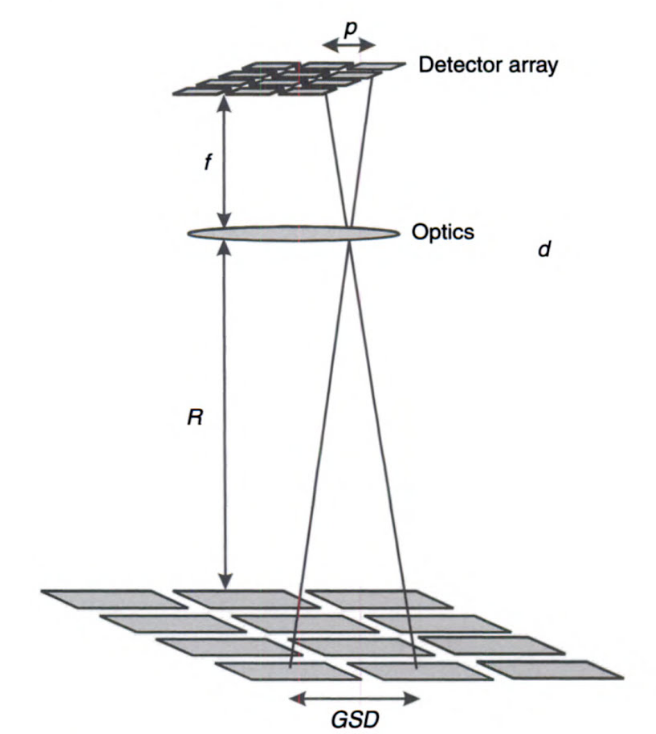
\includegraphics[width=0.7\textwidth]{fig/GSDimage}
  \caption{Ground Sample Distance. From \cite{s}}
  \label{fig:gsd}
\end{figure}


Where $R$ is the distance from the optics to the ground and $W$ is the width of the image in pixels. GSD is illustrated in Figure \ref{fig:gsd}. Equation \ref{gsd1} assumes that the sensor is directed normal to the ground surface. If the sensor is not aligned normal to the ground, the GSD must be expanded for the look angle between the ground and the sensor $\theta$:
\begin{align}
    GSD = \frac{pR}{fW\cos{\theta}}\quad\quad\textrm{[meters/pixel]}
    \label{gsd2}
\end{align}
Where $\theta$ is the angle the sensor is facing with respect to the ground plane. By taking the geometric mean of the horizontal and vertical ground sample distances you get a two-dimensional system GSD\cite{s} factor. \\

To calculate GSD it is assumed that certain camera properties are known and that we have a way to measure or calculate the distance from the object to which we are calculating the GSD. With these pieces of information, it is possible to convert an image from pixels to real life units.